\documentclass[10pt,a4paper,noendnumber=true]{scrartcl}
%german umlauts and localization
\usepackage[utf8]{inputenc} 
\usepackage[T1]{fontenc}
\usepackage[ngerman]{babel}
\usepackage[dvipsnames]{xcolor}
\usepackage{booktabs}
\usepackage{tabularx}

\usepackage{geometry}
\geometry{
	a4paper,
	total={170mm,257mm},
	left=20mm,
	top=20mm,
}

%figures etc.
\usepackage[pdftex]{graphicx}
\usepackage{standalone} %externalize files for faster compilation
\usepackage{float}

%mathematical symbols
\usepackage{latexsym} % special symbols 
\usepackage{amsmath,amssymb,amsthm}
\usepackage{textcomp} % supports the Text Companion fonts, which provide many text symbols (such as baht, bullet, copyright, musicalnote, onequarter, section, and yen)
%fonts:
%\usepackage{txfonts}  %supplies virtual text roman fonts using Adobe Times % needs to be loaded AFTER amsmath (because otherwise \iint is defined twice)
\usepackage{mathrsfs}  % for script-like fonts in math mode
\usepackage{nicefrac} % nice fracs in text

%\usepackage{libertine}
%\usepackage[libertine]{newtxmath}
%\usepackage[sc]{mathpazo}
%\linespread{1.05}

%tables
\usepackage{tabularx}

%units
\usepackage{siunitx}

%tikz
\usepackage{tikz}
\usepackage{tikzscale}
\usepackage{pgfplots} 
\usepackage{pgfgantt}
\usepackage{pdflscape}
\usepackage[european]{circuitikz}
\pgfplotsset{compat=newest} 
\pgfplotsset{plot coordinates/math parser=false}
\usetikzlibrary{shapes.geometric}
\usetikzlibrary{arrows.meta}
\usetikzlibrary{arrows}
\usetikzlibrary{shapes.symbols,shadows}

%bib stuff
\usepackage[draft = false]{hyperref}
\usepackage{csquotes}
\usepackage[backend=biber,style=ieee]{biblatex}
%\addbibresource{bib.bib}

% gescheiter Abstand nach paragraph
\newcommand{\properparagraph}[1]{\paragraph{\textcolor{Emerald}{#1}}\mbox{}\\}
\usepackage[parfill]{parskip}

% für die Auflistung von Vor- und Nachteilen in itemize-Umgebung
\newcommand\pro{\item[$+$]}
\newcommand\con{\item[$-$]}

%nice row vector
\newcommand{\rvect}[1]{\begin{bmatrix} #1 \end{bmatrix}}

%align multi pgfplots
\pgfplotsset{yticklabel style={text width=3em,align=right}}

\usetikzlibrary{external}
\tikzexternalize[optimize=false,prefix=tikz/] % activate!

\usepackage{subfig}
\renewcommand{\arraystretch}{1.6}

\title{Entrepreneurship}
\subtitle{Question Catalogue and Summary}
\author{}


\begin{document}
\maketitle

\section{Question Catalogue}

\subsection{Session 1}

\properparagraph{What is the activity of an entrepreneur according to Jean Baptiste Say?}
\properparagraph{How does Joseph Schumpeter define "`entrepreneurship"'?}
\properparagraph{Please give one example of "`Creative Destruction"' related to entrepreneurship.}
\properparagraph{How was the term "`entrepreneur"' defined according to the synthesis of Terzidis(2017)?}
\properparagraph{What are the key activities of entrepreneurs according to Byers et al. (2011)?}
\properparagraph{What are the personality traits of successful entrepreneurs according to Rauch \& Frese(2007)?}
\properparagraph{What are the career reasons for nascent entrepreneurs according to Carter et al. (2003)?}
\properparagraph{What is the role of entrepreneurship according to the definition of the OECD?}
\properparagraph{Give a definition of the term "`business opportunity"' according to Byers et al. (2011).}
\properparagraph{Please name five of the nine categories of opportunity according to Byers et al. (2011).}
\properparagraph{Name and describe the characteristics of attractive opportunities. Please give an example only for three of these characteristics.}


\subsection{Session 2}
\properparagraph{What is the definition of a firm according Coase (1937)?}
\properparagraph{Please fill with the missing terms on the \autoref{fig:sess2_diagram}: "`The firm as a System"'.}
\begin{figure}[H]
	\centering
	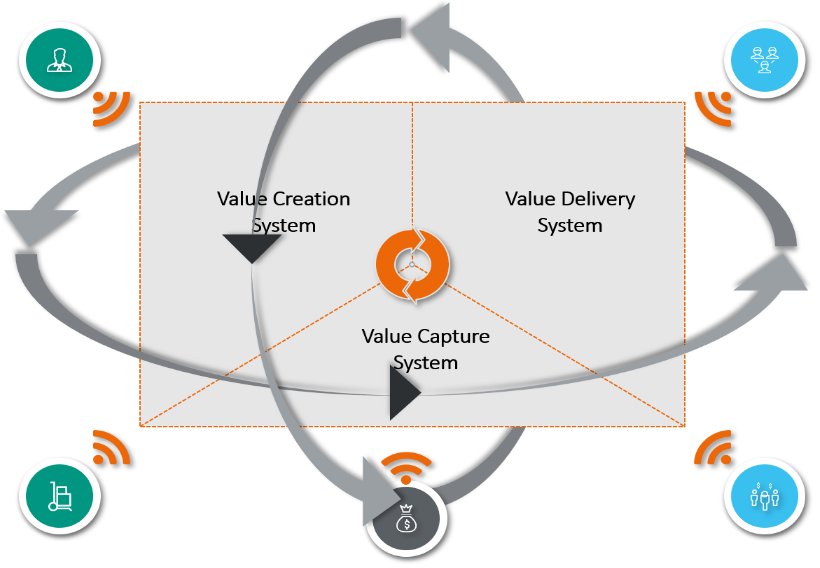
\includegraphics[width = 0.5\textwidth]{img/firm_system}
	\caption{Firm as a System} \label{fig:sess2_diagram}
\end{figure}
\properparagraph{Keeping in mind the concept of the firm as a living system, please give two examples of an "`anabolic process"' (Growth and Change) and two of a "`catabolic process"' (Operation).}
\properparagraph{Give a defintion if the term "`business model"' according to Terzidis(2017).}
\properparagraph{What are business model V4 dimensions according to Al Debei and Avison (2011)?}
\properparagraph{Please name the building blocks of the Business Model Canvas.}
\properparagraph{Name the limitations of the Business Model Canvas.}
\properparagraph{Fill the business model canvas for a daily newspaper!}
\properparagraph{What does strategic management deal with according to Terzidis(2017)?}
\properparagraph{What is an industry according to Dorf \& Byers (2011)?}
\properparagraph{Describe an industry analysis using five steps mentioned in the lecture.}
\properparagraph{Name the four phases in the Industry Lifecycle.}
\properparagraph{What is a sustained competitive advantage according to Barney (1991)?}
\properparagraph{Name the three key principles for strategic positioning (Porter, 2008).}


\subsection{Session 3}
\properparagraph{Please give a definition of market and the actors who determine the market according to Homburg (2017).}
\properparagraph{Give a definition of marketing according to the American Marketing Association.}
\properparagraph{Name the 4 P’s of the Marketing Mix according to Hisrichand Ramadani(2017).}
\properparagraph{What are the five dimensions of value of an offering according to Dorf \& Byers?}
\properparagraph{Please give the definition of a "`job"' and its three characteristics according to the Job to be done theory (Ulwick2016).}
\properparagraph{What are the three steps of the Strategic Marketing Process?}
\properparagraph{What is market segmentation according to Smith (1956)?}
\properparagraph{What are the five stages of innovation diffusion according to Roger (1983) and Moore (1991)?}
\properparagraph{Name 4 methods to estimate the market size.}
\properparagraph{What are the three approaches to determine the price of an offering?}
\properparagraph{What are the four questions asked in the method described by van Westendorp(1976)?}
\properparagraph{Please give the definition of ‘Lean Startup’ presented in the lecture and name the four steps of the lean startup method?}
\properparagraph{Name the six components of the validated learning loop according to Ries(2011).}
\properparagraph{Please give the definition of Minimal Viable Product (MVP) and Pivot given in the lecture? Give one example for each concept.}

\subsection{Session 4}
\properparagraph{What is a patent (definition used in the lecture)?}
\properparagraph{What is meant by "`novelty"' according to German patent law (§3 sentence 1 PatG)?}
\properparagraph{What is meant by "`inventive activity"' according to German patent law (§4 PatG)?}
\properparagraph{Name three opportunities and three risks related to patenting.}
\properparagraph{Name the Success Factors of New Ventures according to Song et al. (2008).}
\properparagraph{Compare market pull to technology push processes by naming five attributes and stating the differences with respect to these attributes.}
\properparagraph{Explain the objective of Intellectual Property.}
\properparagraph{What is a Patent Family? What are the advantages of using a patent family?}
\properparagraph{Describe the Employee Invention act.}

\subsection{Session 5}
\properparagraph{Please name the six principles of effective management according to Malik (2006) and explain each one in your own words.}
\properparagraph{What are the five tasks of effective leadership according to Malik (2006)?}
\properparagraph{What does SMART stand for in the context of goals?}
\properparagraph{Please define the term "`decision"' using the definitions of Mintzberg (1976) and the Gabler business dictionary (Wirtschaftslexikon).}
\properparagraph{What are the main three phases of the decision-making process according toSimon (1965, 1977)and Mintzberg (1976)?}
\properparagraph{Please name the 7 stages of a decision-making process according to Malik (2006).}
\properparagraph{What are the seven tools of effective leadership according to Malik(2006)?}
\properparagraph{Please name and explain thefiveapproachestoleadership.}
\properparagraph{Summarize in your own words the empirical distillate of theories and studies of leadership.}
\properparagraph{Identify the types of competences mentioned on the lecture and give three examples for each one.}

\newpage

\section{Summary}
\end{document}

